\myparagraph{
    \begin{tcolorbox}[colback=blue!5!white, colframe=blue!75!black]
        Il Virtual Proxy è un Proxy per l'oggetto "reale", questo proxy virtuale
        materializza l'oggetto solo la prima volta a cui gli si fa riferimento,
        rappresentandoli come oggetti leggeri che fungono da sostituto all'oggetto
        reale (che possono essere più pesanti).
    \end{tcolorbox}

    In sostanza, il Virtual Proxy funge da sostituto dell'oggetto reale, ma in un formato
    più leggero. Sarà questo sostituto a gestire l'accesso all'oggetto reale e a caricarlo
    in memoria solo quando è strettamente necessario, in modo da evitare materializzazioni
    inutili.

    \begin{wrapfigure}{r}{0.55\textwidth}
        \begin{center}
          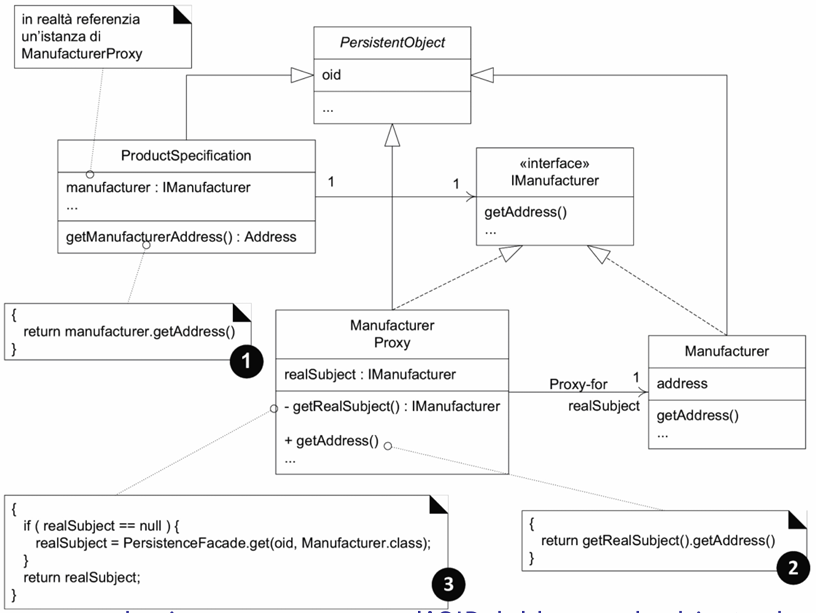
\includegraphics[width=0.55\textwidth]{Esercitazione - Design Patterns/Virtual Proxy.png}
        \end{center}
      \end{wrapfigure}
    
    \hbadness=2000
    Nell'esempio, Manufacturer è il nostro oggetto reale, \textbf{Manufacturer Proxy} è il suo \textbf{Virtual Proxy}, quindi
    un suo sostituto che ne gestisce l'accesso e stabilisce se caricarlo in memoria o meno. L'interfaccia comune \textit{IManufacturer}
    permette al client di interagire con il Virtual Proxy senza sapere che si tratta di un suo sostituto.

    Bisogna fare una considerazione, dato che parliamo di materializzazione ovviamente è coinvolto anche il pattern \textbf{DatabaseMapper},
    che in questo esempio è rappresentato dalla classe \textbf{ProductSpecification}, infatti questa crea un'istanza di \textit{IManufacturer},
    con lo scopo di decidere quali oggetti materializzare subito e a quali invece può ritardare questo processo. Si parla quindi di
    \textbf{Eager} e \textbf{Lazy Materialization}.

    \newpage
}